\documentclass[aspectratio=169,10pt]{beamer}

% Theme & Styling
\usetheme{Madrid}
\usecolortheme{whale}

% ITB Color Palette
\definecolor{ITBblue}{RGB}{0, 75, 141}
\definecolor{ITBgold}{RGB}{200, 150, 40}
\setbeamercolor{structure}{fg=ITBblue}
\setbeamercolor{title}{fg=white,bg=ITBblue}
\setbeamercolor{frametitle}{fg=white,bg=ITBblue}
\setbeamercolor{block title}{fg=white,bg=ITBblue}
\setbeamercolor{block body}{bg=ITBblue!8}

% Packages
\usepackage[utf8]{inputenc}
\usepackage{amsmath,amssymb}
\usepackage{graphicx}
\usepackage{hyperref}
\usepackage{multimedia}

\title[MA1101 Matematika I]{MA1101 Matematika I --- Bab 2: Turunan}
\subtitle{Subtopik 2.7: Turunan Implisit (\textit{Implicit Differentiation})}
\author[FMIPA ITB]{Tim Pengajar MA1101}
\institute[ITB]{Fakultas Matematika dan Ilmu Pengetahuan Alam\\Institut Teknologi Bandung}
\date{Semester 1 Tahun Akademik 2026/2027}

\begin{document}

% -------------------------------------------------------------
% Slide 1: Judul
% -------------------------------------------------------------
\begin{frame}
    \titlepage
\end{frame}

% -------------------------------------------------------------
% Slide 2: Tantangan Sokratik (The Pique)
% -------------------------------------------------------------
\begin{frame}{Tantangan Awal: Eksplisit vs Implisit}
    \begin{columns}[T]
        \begin{column}{0.55\textwidth}
            \begin{block}{Fungsi Eksplisit vs Hubungan Implisit}
                \begin{itemize}
                    \item \textbf{Eksplisit}: $y = f(x)$, variabel $y$ terisolasi di satu ruas (lolos uji garis vertikal).
                    \item \textbf{Implisit}: $F(x, y) = C$, variabel $x$ dan $y$ terikat bersama (misal: lingkaran $x^2 + y^2 = 25$).
                \end{itemize}
            \end{block}

            \vspace{0.2cm}
            \begin{alertblock}{Pertanyaan Sokratik}
                Kurva lingkaran \textbf{bukan sebuah fungsi} karena satu nilai $x$ memiliki dua nilai $y$.
                Bagaimana cara kita menghitung gradien garis singgung $\frac{dy}{dx}$ di titik $P(3, 4)$ tanpa harus mengisolasi $y = \pm\sqrt{25 - x^2}$?
            \end{alertblock}
        \end{column}

        \begin{column}{0.42\textwidth}
            \centering
            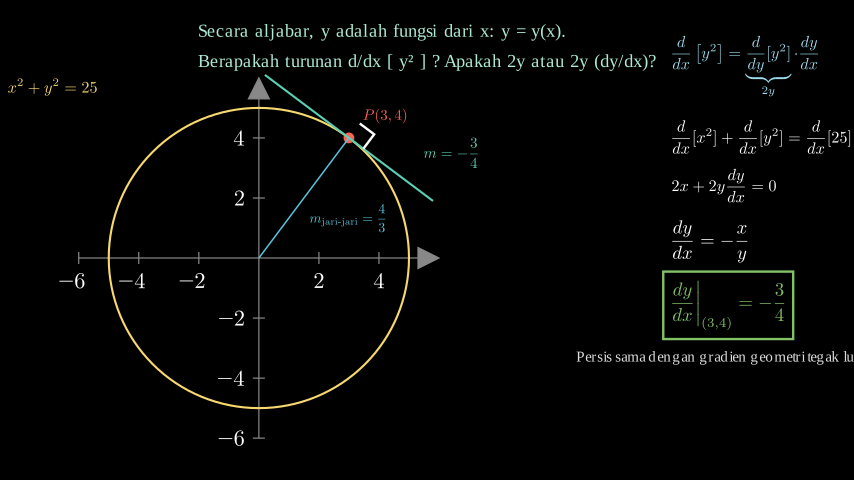
\includegraphics[height=0.52\textheight]{keyframe_implisit.png}\\
            \vspace{0.1cm}
            {\scriptsize \textit{Lingkaran $x^2 + y^2 = 25$ dan Titik $P(3, 4)$}}
        \end{column}
    \end{columns}
\end{frame}


% -------------------------------------------------------------
% Slide 3: Animasi Video Interaktif
% -------------------------------------------------------------
\begin{frame}{Simulasi Dinamis: Turunan Implisit \& Geometri}

    \centering
    % Embedded video untuk presenter (Pympress / PDFPC / Okular)
    \movie[width=9.6cm,height=5.4cm,poster,showcontrols=true]{%
        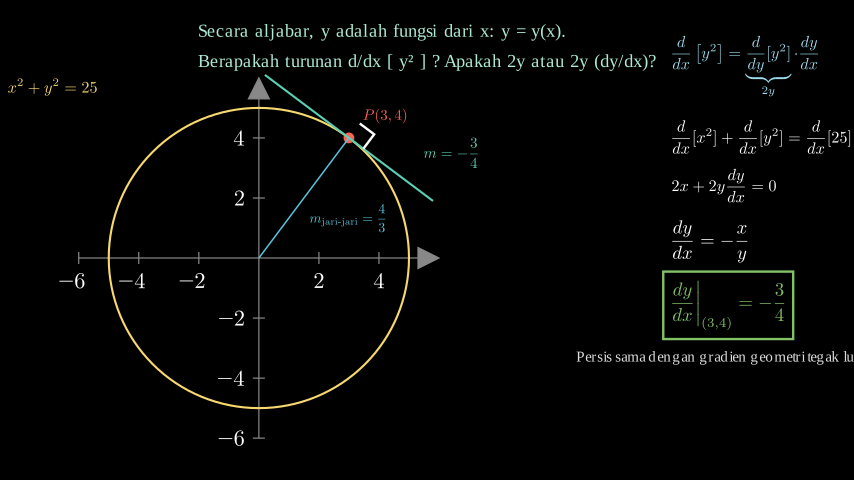
\includegraphics[height=0.55\textheight]{keyframe_implisit.png}%
    }{ImplicitDifferentiationScene.ogv}
    
    \vspace{0.2cm}
    \href{file:ImplicitDifferentiationScene.mp4}{%
        \beamergotobutton{\normalsize $\blacktriangleright$ Putar Video (\texttt{ImplicitDifferentiationScene.mp4})}%
    }
    
    \vspace{0.15cm}
    {\scriptsize \textit{Klik poster untuk memutar langsung di Pympress/Okular, atau klik tombol untuk membuka di MPV/VLC.}}
\end{frame}

% -------------------------------------------------------------
% Slide 4: Kristalisasi Matematis Formal
% -------------------------------------------------------------
\begin{frame}{Penurunan Matematis: Mengapa Muncul Aturan Rantai?}
    \begin{columns}[T]
        \begin{column}{0.48\textwidth}
            \begin{block}{1. Kunci Utama: $y$ adalah Fungsi dari $x$}
                Ingat bahwa $y = y(x)$. Menurut \textbf{Aturan Rantai}:
                \[
                    \frac{d}{dx}\left[ y^n \right] = n y^{n-1} \cdot \mathbf{\frac{dy}{dx}}
                \]
                Contoh: $\frac{d}{dx}[y^2] = 2y \frac{dy}{dx}$.
            \end{block}

            \begin{block}{2. Diferensialkan Kedua Ruas terhadap $x$}
                \[
                    \frac{d}{dx}[x^2] + \frac{d}{dx}[y^2] = \frac{d}{dx}[25]
                \]
                \[
                    2x + 2y \frac{dy}{dx} = 0
                \]
            \end{block}
        \end{column}

        \begin{column}{0.48\textwidth}
            \begin{exampleblock}{3. Isolasi $\frac{dy}{dx}$}
                Pindahkan suku tanpa $\frac{dy}{dx}$ ke ruas kanan:
                \[
                    2y \frac{dy}{dx} = -2x \implies \mathbf{\frac{dy}{dx} = -\frac{x}{y}}
                \]
            \end{exampleblock}

            \begin{alertblock}{4. Evaluasi di Titik $P(3, 4)$}
                Substitusi $x = 3$ dan $y = 4$:
                \[
                    m_{\text{singgung}} = \left. \frac{dy}{dx} \right|_{(3, 4)} = -\frac{3}{4}
                \]
                Persis tegak lurus dengan jari-jari $m = \frac{4}{3}$ karena $\left(-\frac{3}{4}\right)\left(\frac{4}{3}\right) = -1$!
            \end{alertblock}
        \end{column}
    \end{columns}
\end{frame}

% -------------------------------------------------------------
% Slide 5: Latihan Mandiri (Soal UTS / Purcell)
% -------------------------------------------------------------
\begin{frame}{Latihan Terarah: Kurva Berderajat Lebih Tinggi}
    \begin{block}{Contoh Soal (Folium Descartes)}
        Diberikan persamaan kurva $x^3 + y^3 - 6xy = 0$.
        Tentukan persamaan garis singgung pada kurva tersebut di titik $(3, 3)$.
    \end{block}

    \pause
    \begin{columns}[T]
        \begin{column}{0.48\textwidth}
            \textbf{Langkah 1: Diferensialkan Implisit}
            Ingat aturan hasil kali untuk suku $6xy$:
            \[
                \frac{d}{dx}[6xy] = 6\left( 1 \cdot y + x \frac{dy}{dx} \right)
            \]
            Sehingga persamaan menjadi:
            \[
                3x^2 + 3y^2 \frac{dy}{dx} - 6y - 6x \frac{dy}{dx} = 0
            \]
            \[
                (3y^2 - 6x)\frac{dy}{dx} = 6y - 3x^2
            \]
        \end{column}

        \begin{column}{0.48\textwidth}
            \textbf{Langkah 2: Evaluasi di Titik $(3, 3)$}
            \[
                \frac{dy}{dx} = \frac{6y - 3x^2}{3y^2 - 6x} = \frac{2y - x^2}{y^2 - 2x}
            \]
            Substitusi $x = 3, y = 3$:
            \[
                m = \frac{2(3) - (3)^2}{(3)^2 - 2(3)} = \frac{6 - 9}{9 - 6} = \frac{-3}{3} = \mathbf{-1}
            \]
            \textbf{Langkah 3: Persamaan Garis Singgung}
            \[
                y - 3 = -1(x - 3) \implies \mathbf{y = -x + 6}
            \]
        \end{column}
    \end{columns}
\end{frame}

\end{document}
